%----------------------------------------------------------------------------------------
%	PACKAGES AND DOCUMENT CONFIGURATIONS
%----------------------------------------------------------------------------------------

\documentclass[10pt,a4paper]{article}

% Adjusting margins to personal my need
\addtolength{\oddsidemargin}{-.5in}
\addtolength{\evensidemargin}{-.5in}
\addtolength{\textwidth}{1in}
\addtolength{\topmargin}{-.5in}
\addtolength{\textheight}{1in}

% Graphics
\usepackage{caption}
\usepackage{subcaption}
\usepackage{graphicx}
\usepackage{float}
\graphicspath{{figures/}}

% Math
\usepackage{amssymb}
\usepackage{amsmath} % Required for some math elements 

% Other
\usepackage{algorithmic}
\usepackage{array}
\usepackage{lipsum}
\usepackage{hyperref}
\usepackage{minted}




%----------------------------------------------------------------------------------------
%	MAIN PART
%----------------------------------------------------------------------------------------
\begin{document}

\title{Analysing the saleability of cars through Bayesian Networks} % Title
\author{Simone Montali - 983806}
\date{May 2021} % Date for the report
\maketitle % Inserts the title, author and date




%----------------------------------------------------------------------------------------
%	Abstract
%----------------------------------------------------------------------------------------
\begin{abstract}
\normalsize
Provided with a \textbf{dataset} consisting of data about several cars, this paper first tries to infer a \textbf{Bayesian Network} that accurately describes the problem and its probabilistic background, then, using the generated network, provides an analysis on the \textbf{interest} generated by the car for future saleability with respect to different features of the car. The inference is first calculated with \textbf{variable elimination}, then an approximation through \textbf{Rejection Sampling} and \textbf{Likelihood Weighting} is compared to the initial results.

\end{abstract}

%----------------------------------------------------------------------------------------
%	Table of Content
%----------------------------------------------------------------------------------------
\setcounter{tocdepth}{2}
\tableofcontents


\clearpage

%----------------------------------------------------------------------------------------
%	Main Part
%----------------------------------------------------------------------------------------
\section{Introduction}
\label{sec:introduction}

The car market has been, in the last century, subject to a constant and strong growth. Nowadays, all kinds of features and gadgets have been added to all the car segments, from small city vehicles to luxury ones. Sometimes, though, to get a better grip on what the people prefer, abstracting from buttons, touch screens and custom horn sounds, \textbf{a simplicistic vision is preferrable}. This is the reason why the analysis of a rather simple dataset through probabilistic reasoning could actually produce really interesting insights on how cars are chosen by the public.
\section{Dataset}
\label{sec:dataset}
This dataset \href{https://archive.ics.uci.edu/ml/datasets/Car+Evaluation}{(click here)} was created in 1997 by two researchers of the Jožef Stefan Institute in Ljubljana, Slovenija to demonstrate a qualitative multi-criteria decision analysis (MCDA) method for decision making, DEX. The provided data consists of the classification of different features in $\approx 1800$ cars. The target attribute is the \textbf{car acceptability}, a measure of the interest in the car demonstrated by the public. It is obvious that this dataset is a strong simplification of what actually happens when buying a car, and the fact that it was artificially crafted by someone doesn't help. Nonetheless, it perfectly fits the needs of a project like this one. The features that are stated for each car are the following: the buying price, the maintenance price, the number of doors, the seats, the size of the lug boot, the safety. Obviously, the numeric attributes like the prices are \textbf{bucketized}. Therefore, the final attribute list is the following:
\begin{center}
\begin{tabular}{|l|l|}
\hline
\textbf{attribute} & \textbf{values}\\
\hline
acceptability & \textit{unacc, acc, good, vgood}\\
\hline
buying & \textit{vhigh, high, med, low}\\
\hline
maint & \textit{vhigh, high, med, low}\\
\hline
doors & \textit{2,3,4,5more}\\
\hline
people & \textit{2,4,more}\\
\hline
lug\_boot & \textit{small, med, big}\\
\hline
safety & \textit{low, med, high}\\
\hline
\end{tabular}
\end{center}
The data is in CSV format, so a car in the dataset looks like this:
\begin{center}
    \texttt{vhigh,vhigh,3,2,small,high,unacc}
\end{center}
\section{Bayesian Network}
\label{sec:bayesiannet}
Bayesian Networks allow us to \textbf{economically encode a probability distribution} over a set of variables, stating the \textbf{conditional independencies} across the different variables, a rather interesting notion in the analysis of this problem. They are a sufficient and compact specification of the full joint distribution. No Bayesian Network of the problem was available, but luckily the Python library \texttt{pgmpy} has exactly what is needed for us to obtain the network and its \textit{Conditional Probability Tables} from the dataset.
\subsection{Structure learning}
To learn the model structure, i.e. a Directed Acyclic Graph, there are \textbf{two different families of techniques} that can be chosen: the constraint-based approaches, which search for a graph structure satisfying the independence assumptions that we observe in the empirical distribution; and the score-based approaches, which define an objective function for different models, and then search for a high-scoring model. \cite{book:probgraphmod}
The approach I chose is the latter, needing a \textbf{scoring function} $s_D: M \rightarrow \mathbb{R}$, which maps a model $x \in M$ to a real score, based on how well it fits to the given dataset. Then, a search strategy traverses the space of all possible models and selects the one with optimal score. Several scoring functions are available, such as \textit{BDeu}, \textit{K2} and \textit{BIC}. The last one, \textit{Bayesian Information Criterion}, is a good asymptotic approximation of the likelihood of the training data. After having defined a scoring function, we can choose different search strategies, usually \textit{local searches}, i.e. iterative search algorithms that keep improving a solution until a local maxima is reached. The algorithm I chose is \textbf{Hill Climb Search}, a rather simple algorithm that is able to explore the search space (while still not being extraordinarily performant) and find a good solution. 
To learn the network structure through \texttt{pgmpy}, we'll first have to import the data in a Pandas DataFrame:
\begin{minted}{python}
import pgmpy
import pandas as pd
cars_data = pd.read_csv('data/car.data', names=["Buying", "Maintenance",
"Doors", "People", "LugBoot", "Safety", "Acceptability"])
\end{minted}
Then, we'll just use \textit{pgmpy}'s \texttt{HillClimbSearch} with a \texttt{BicScore}:
\begin{minted}{python}
from pgmpy.estimators import HillClimbSearch
from pgmpy.estimators import BicScore

hc = HillClimbSearch(cars_data, scoring_method=BicScore(cars_data))
best_model = hc.estimate()
\end{minted}

\subsubsection{Learned graph}
After some instants, the search finds its best guess of model. We can therefore print its \textbf{edges} with \texttt{best\_model.edges()} obtaining the following result:
\begin{center}
\texttt{[('Buying', 'Maintenance'), ('Safety', 'People'), ('Safety', 'LugBoot'), ('Acceptability', 'Safety'), ('Acceptability', 'People'), ('Acceptability', 'Buying'), ('Acceptability', 'Maintenance'), ('Acceptability', 'LugBoot')]}
\end{center}
which, in a more graphically appealing way, is the following graph:
\begin{figure}[ht]
    \centering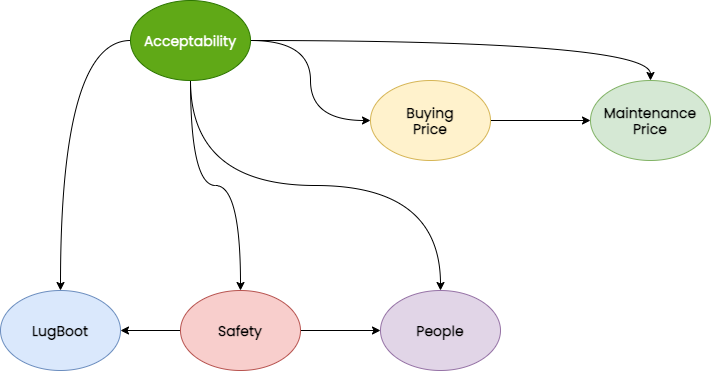
\includegraphics[width=0.8\linewidth]{figures/DAG.png}
    \caption{Bayesian network for the cars dataset}
    \label{fig:errors}
\end{figure}

\subsection{Parameter learning}
Now that we've found a good structure for our graph, we'll have to find the values of the Conditional Probability Distributions. The library \texttt{pgmpy} is a great tool for this task too. If one would have to find a solution for this problem, it would be pretty natural to think about the \textbf{relative frequencies} of the variable states. This approach is, basically, what \textit{Maximum Likelihood Estimation} does: as seen in section 17.1 of \cite{book:probgraphmod}, the likelihood function for a given choice of parameters $\theta$ is the probability the model assigns the training data:
\begin{equation}
L(\boldsymbol{\theta}: \mathcal{D})=\prod_{m} P(\xi[m]: \boldsymbol{\theta})
\end{equation}
In other words, we want to maximize the probability $P(data|model)$. This, in practice, is done by computing the state counts and dividing by the conditional sample size.
MLE has a high possibility of overfitting on small very datasets. This, fortunately, is not our case, and we would otherwise have needed a different estimator, like Bayesian Parameter Estimation. We can estimate the parameters and print the CPDs with:
\begin{minted}{python}
from pgmpy.models import BayesianModel
from pgmpy.estimators import MaximumLikelihoodEstimator

bayesian_model = BayesianModel(best_model.edges())
bayesian_model.fit(cars_data, estimator=MaximumLikelihoodEstimator)
for cpd in bayesian_model.get_cpds():
    print(cpd)
\end{minted}
Having finally built our full joint distribution, we can proceed and \textbf{answer some questions through inference}.
\section{Exact inference}
\label{sec:exactinference}
\subsection{Theoretical background}
\subsubsection{Summing out}
At this moment, it is very well clear that the basic task for a probabilistic inference system would be, as the word says, performing \textbf{inference}, i.e. computing the posterior probability for a set of query variables, given some observed event in the form of evidence variable. Moreover, it is clear that by \textbf{summing out} the probabilities from the full joint distribution, we are able to compute any conditional probability. More specifically, a query $\mathbf{P}(X \mid \mathbf{e})$ can be always computed as:
\begin{equation}
    \mathbf{P}(X \mid \mathbf{e})=\alpha \mathbf{P}(X, \mathbf{e})=\alpha \sum_{\mathbf{y}} \mathbf{P}(X, \mathbf{e}, \mathbf{y})
\end{equation}
\subsubsection{Variable elimination}
A crucial improvement in this algorithm is provided by \textbf{variable elimination}, which we can simplify as a form of \textbf{dynamic programming}, in which the factors get saved into an array to avoid recomputing the same thing multiple times.
\subsection{Variable elimination with pgmpy}
As always, \texttt{pgmpy} allows us to do so in a straightforward way:
\begin{minted}{python}
from pgmpy.inference import VariableElimination
exact_inference = VariableElimination(bayesian_model)
\end{minted}
Having instantiated the \texttt{exact\_inference} object, we can then call queries on it. For example, a nice question to ask would be:
\begin{center}
    \textit{Is maintenance harder for 2-seaters than for family cars?}
\end{center}
With just two lines of code, we can produce the probability tables for this query:
\begin{minted}{python}
print(exact_inference.query(["Maintenance"],{'People':"2"}))
print(exact_inference.query(["Maintenance"],{'People':"4"}))
\end{minted}
\begin{center}
\begin{figure}[H]
\subfloat[Maintenance on 2-seaters]{
    \begin{tabular}{|l|l|}
        \hline
        \textbf{Maintenance level}&\textbf{Probability}\\
        \hline
        very high & 0.2975 \\
        \hline
        high & 0.2595 \\
        \hline
        medium & 0.2215 \\
        \hline
        low & 0.2215 \\
        \hline
    \end{tabular}
}
\subfloat[Maintenance on 4-seaters]{
    \begin{tabular}{|l|l|}
        \hline
        \textbf{Maintenance level}&\textbf{Probability}\\
        \hline
        very high & 0.2256 \\
        \hline
        high & 0.2450 \\
        \hline
        medium & 0.2646 \\
        \hline
        low & 0.2648 \\
        \hline
    \end{tabular}
}
\end{figure}
\end{center}
It looks like sport cars are not the best kind of choice if you want to stay cheap on oil and filters.
\begin{center}
    \textit{Are cars with high maintenance safe?}
    \end{center}
\begin{center}
    \begin{tabular}{|l|l|}
        \hline
        \textbf{Safety}&\textbf{Probability}\\
        \hline
        high & 0.2793 \\
        \hline
        medium & 0.3240 \\
        \hline
        low & 0.3967 \\
        \hline
    \end{tabular}
    \end{center}

It looks like they are not!

\section{Evaluation}
\label{sec:evaluation}
\lipsum[8]

\subsection{Subsection}
\lipsum[8]

\subsection{Subsection}
\lipsum[8]
\section{Conclusion}
\label{sec:conclusion}
We have seen how Bayesian Networks can prove themselves as an extraordinary tool to summarize complex probabilistic domains. This could step up the process of decision making in multiple situations, while still being intrinsically elegant and simple. Tools like \texttt{pgmpy} make the whole job a breeze: the programmer just has to think about the data, the computer will do the rest. That probably is how a truly \textit{intelligent} system would perform. We have then seen how exact inference is - while still being computationally heavy - a great tool, and, moreover, how we can use \textbf{approximate inference} to achieve similar results with less, less work. 

\clearpage

%----------------------------------------------------------------------------------------
%	Appendix
%----------------------------------------------------------------------------------------
\appendix
\section{Report Instructions}
\label{sec:appendix}
Your technical report should focus on the work that you have done in the project. Additionally, you should also provide brief descriptions of the components/parts that you rely on in your work. Make sure to describe everything in your own words!

This template includes the basic structure for your final technical report. You should keep the overall structure by not changing the \textit{sections}. You can still adjust the structure a bit by adding \textit{subsections}. In the appendix, you find these instructions as well as some \LaTeX{} examples. Before you hand in the report, makes sure you have deleted all \textit{lipsum} fillings and the instructions/examples from the appendix.



\subsection*{Abstract}
\begin{itemize}
    \item Maximum length: 10 lines!
    \item Important: Do not put references into the abstract
    \item Content of the abstract:
        \begin{itemize}
        \item Punchline
        \item Introduction. Why should I care?
        \item What is the problem? How did you tackled the problem?
        \item How did you go about doing the research that follows from your idea?
        \item What’s the key impact of your research?
    \end{itemize}
\end{itemize}


\subsection*{Main Part}
\begin{itemize}
    \item Main Part consists of 6 sections: Introduction, Dataset, Methodology, Methods, Evaluation, Conclusion
    \item Maximum(!) length without figures/tables: 3 pages
    \item Suggested length with figures/tables: 4 pages
    \item Additional content should be put in appendix.
    \item Content in appendix must not be required to understand the main part.
\end{itemize}


\subsubsection*{Introduction}
\begin{itemize}
    \item General introduction of the problem that you were trying to solve. 
    \item What is the brief problem description? 
    \item Why is it important/interesting/challenging? 
\end{itemize}


\subsubsection*{Dataset}
\begin{itemize}
    \item General description of the dataset that you were using. 
    \item Important details about the dataset. 
    \item What modifications/preprocessing did you do (if any)? Only mention things here that you used for all of your methods later, e.g., resizing, cropping, or combining images. 
    \item What are the details of the final modified dataset that you used. 
\end{itemize}


\subsubsection*{Methodology}
\begin{itemize}
    \item What do you want to do? What kind of problem is it?
    \item What is the dataset?
    \item What is the input of each part?
    \item What is the output of each part?
    \item What is/are the metric/s you want to evaluate on?
\end{itemize}
% protocol, metric, etc.

Remember: show your reader the wall before you begin to examine the bricks.

% Methodology (protocol, metric, etc.)
% a. If you tackled the project by solving two problems, describe the two methodologies here.

\subsubsection*{Methods}
\begin{itemize}
    \item Methods that you tried
\end{itemize}


\subsubsection*{Evaluation}
\begin{itemize}
    \item Evaluation of the methods with the described metric
    \item Comparison of your methods
\end{itemize}


\subsubsection*{Conclusion}
\begin{itemize}
    \item Conclusion of your work
    \item What is working? What does not work? Where could your methods be improved?
\end{itemize}


\subsection*{Appendix}
\begin{itemize}
    \item Additional content can be put in the appendix.
    \item Appendix must not be required to understand the main part.
    \item You should still not dump all images and data into the appendix. You should make a selection of useful additions.
    \item Appendix is not required.
\end{itemize}


\clearpage
\section{\LaTeX{} Examples}
The following examples should help you to write your technical report using \LaTeX{}. You'll find here the examples of tables, figures, citations and references. For other features of \LaTeX{}, see tutorials on \href{https://www.overleaf.com/learn}{\textbf{Overleaf}} or use this \href{https://wch.github.io/latexsheet/}{\textbf{cheatsheet}}. To work with this template, download its entire folder (including /sections, /bibliography and /figures), and run your \LaTeX{} editor like \href{https://www.overleaf.com}{\textbf{Overleaf}}.


\subsection*{Example Citation}
Example of citation: \cite{Smith_2013} and \cite{Smith_2012}. 


\subsection*{Example References}
Example of table reference: see Table \ref{tab:example}. \\
Example of equation reference: see Equation \eqref{eq:emc}. \\
Example of reference to Section \ref{sec:methods}. \\
Example of reference to Subsection \ref{sec:dataset:subsection}. \\
Example of figure reference: see Figure \ref{fig:example}.\\
Example of subfigure reference: see Figure \ref{fig:multiple:example11}.\\


\subsection*{Example list}
\begin{itemize}
\item Bullet point one
\item Bullet point two
\item Nested list items:
\begin{itemize}
\item Nested item one
\item Nested item two
\end{itemize}
\end{itemize}

\subsection*{Enumerations}
\begin{enumerate}
\item Numbered list item one
\item Numbered list item two
\item Nested list items:
\begin{enumerate}
\item Nested item one
\item Nested item two
\end{enumerate}
\end{enumerate}


\subsection*{Example Table}

\begin{table}[h] 
\centering
\begin{tabular}{l l l}
\hline
\textbf{Treatments} & \textbf{Response 1} & \textbf{Response 2}\\
\hline
Treatment 1 & 0.0003262 & 0.562 \\
Treatment 2 & 0.0015681 & 0.910 \\
Treatment 3 & 0.0009271 & 0.296 \\
\hline
\end{tabular}
\caption{Table caption}
\label{tab:example}
\end{table}



\subsection*{Example Equation}
Equations within the text: $e = mc^2$. Equation with label on its own line:
\begin{equation} \label{eq:emc}
    e = mc^2
\end{equation}




\subsection*{Example Figures}

\begin{figure}[ht]
    \centering
\includegraphics[width=0.4\linewidth]{placeholder}
    \caption{An example of simple figure.}
    \label{fig:example}
\end{figure}

\begin{figure}[ht]
    \centering
    \begin{subfigure}[t]{0.4\textwidth}
        \centering
\includegraphics[width=1\linewidth]{placeholder}
        \caption{An example of multiple figures in one frame.}
        \label{fig:multiple:example11}
    \end{subfigure}
    %
    \begin{subfigure}[t]{0.4\textwidth}
        \centering
\includegraphics[width=1\linewidth]{placeholder}
        \caption{Next subfigure.}
        \label{fig:multiple:example12}
    \end{subfigure}
    %
    \\
    \begin{subfigure}[t]{0.4\textwidth}
        \centering
\includegraphics[width=1\linewidth]{placeholder}
        \caption{Subfigure on another line.}
        \label{fig:multiple:example21}
    \end{subfigure}
    %
    \begin{subfigure}[t]{0.4\textwidth}
        \centering
\includegraphics[width=1\linewidth]{placeholder}
        \caption{Yet another subfigure.}
        \label{fig:multiple:example22}
    \end{subfigure}
    \caption{More figures in appendix.}
    \label{fig:multiple}
\end{figure}

%----------------------------------------------------------------------------------------
%	Bibliography
%----------------------------------------------------------------------------------------
\clearpage
\bibliography{bibliography/sample}{}
\bibliographystyle{plain}

\end{document}